% Options for packages loaded elsewhere
\PassOptionsToPackage{unicode}{hyperref}
\PassOptionsToPackage{hyphens}{url}
%
\documentclass[
]{article}
\usepackage{lmodern}
\usepackage{amssymb,amsmath}
\usepackage{ifxetex,ifluatex}
\ifnum 0\ifxetex 1\fi\ifluatex 1\fi=0 % if pdftex
  \usepackage[T1]{fontenc}
  \usepackage[utf8]{inputenc}
  \usepackage{textcomp} % provide euro and other symbols
\else % if luatex or xetex
  \usepackage{unicode-math}
  \defaultfontfeatures{Scale=MatchLowercase}
  \defaultfontfeatures[\rmfamily]{Ligatures=TeX,Scale=1}
\fi
% Use upquote if available, for straight quotes in verbatim environments
\IfFileExists{upquote.sty}{\usepackage{upquote}}{}
\IfFileExists{microtype.sty}{% use microtype if available
  \usepackage[]{microtype}
  \UseMicrotypeSet[protrusion]{basicmath} % disable protrusion for tt fonts
}{}
\makeatletter
\@ifundefined{KOMAClassName}{% if non-KOMA class
  \IfFileExists{parskip.sty}{%
    \usepackage{parskip}
  }{% else
    \setlength{\parindent}{0pt}
    \setlength{\parskip}{6pt plus 2pt minus 1pt}}
}{% if KOMA class
  \KOMAoptions{parskip=half}}
\makeatother
\usepackage{xcolor}
\IfFileExists{xurl.sty}{\usepackage{xurl}}{} % add URL line breaks if available
\IfFileExists{bookmark.sty}{\usepackage{bookmark}}{\usepackage{hyperref}}
\hypersetup{
  pdftitle={Data 622 HW 1},
  pdfauthor={Monu Chacko},
  hidelinks,
  pdfcreator={LaTeX via pandoc}}
\urlstyle{same} % disable monospaced font for URLs
\usepackage[margin=1in]{geometry}
\usepackage{color}
\usepackage{fancyvrb}
\newcommand{\VerbBar}{|}
\newcommand{\VERB}{\Verb[commandchars=\\\{\}]}
\DefineVerbatimEnvironment{Highlighting}{Verbatim}{commandchars=\\\{\}}
% Add ',fontsize=\small' for more characters per line
\usepackage{framed}
\definecolor{shadecolor}{RGB}{248,248,248}
\newenvironment{Shaded}{\begin{snugshade}}{\end{snugshade}}
\newcommand{\AlertTok}[1]{\textcolor[rgb]{0.94,0.16,0.16}{#1}}
\newcommand{\AnnotationTok}[1]{\textcolor[rgb]{0.56,0.35,0.01}{\textbf{\textit{#1}}}}
\newcommand{\AttributeTok}[1]{\textcolor[rgb]{0.77,0.63,0.00}{#1}}
\newcommand{\BaseNTok}[1]{\textcolor[rgb]{0.00,0.00,0.81}{#1}}
\newcommand{\BuiltInTok}[1]{#1}
\newcommand{\CharTok}[1]{\textcolor[rgb]{0.31,0.60,0.02}{#1}}
\newcommand{\CommentTok}[1]{\textcolor[rgb]{0.56,0.35,0.01}{\textit{#1}}}
\newcommand{\CommentVarTok}[1]{\textcolor[rgb]{0.56,0.35,0.01}{\textbf{\textit{#1}}}}
\newcommand{\ConstantTok}[1]{\textcolor[rgb]{0.00,0.00,0.00}{#1}}
\newcommand{\ControlFlowTok}[1]{\textcolor[rgb]{0.13,0.29,0.53}{\textbf{#1}}}
\newcommand{\DataTypeTok}[1]{\textcolor[rgb]{0.13,0.29,0.53}{#1}}
\newcommand{\DecValTok}[1]{\textcolor[rgb]{0.00,0.00,0.81}{#1}}
\newcommand{\DocumentationTok}[1]{\textcolor[rgb]{0.56,0.35,0.01}{\textbf{\textit{#1}}}}
\newcommand{\ErrorTok}[1]{\textcolor[rgb]{0.64,0.00,0.00}{\textbf{#1}}}
\newcommand{\ExtensionTok}[1]{#1}
\newcommand{\FloatTok}[1]{\textcolor[rgb]{0.00,0.00,0.81}{#1}}
\newcommand{\FunctionTok}[1]{\textcolor[rgb]{0.00,0.00,0.00}{#1}}
\newcommand{\ImportTok}[1]{#1}
\newcommand{\InformationTok}[1]{\textcolor[rgb]{0.56,0.35,0.01}{\textbf{\textit{#1}}}}
\newcommand{\KeywordTok}[1]{\textcolor[rgb]{0.13,0.29,0.53}{\textbf{#1}}}
\newcommand{\NormalTok}[1]{#1}
\newcommand{\OperatorTok}[1]{\textcolor[rgb]{0.81,0.36,0.00}{\textbf{#1}}}
\newcommand{\OtherTok}[1]{\textcolor[rgb]{0.56,0.35,0.01}{#1}}
\newcommand{\PreprocessorTok}[1]{\textcolor[rgb]{0.56,0.35,0.01}{\textit{#1}}}
\newcommand{\RegionMarkerTok}[1]{#1}
\newcommand{\SpecialCharTok}[1]{\textcolor[rgb]{0.00,0.00,0.00}{#1}}
\newcommand{\SpecialStringTok}[1]{\textcolor[rgb]{0.31,0.60,0.02}{#1}}
\newcommand{\StringTok}[1]{\textcolor[rgb]{0.31,0.60,0.02}{#1}}
\newcommand{\VariableTok}[1]{\textcolor[rgb]{0.00,0.00,0.00}{#1}}
\newcommand{\VerbatimStringTok}[1]{\textcolor[rgb]{0.31,0.60,0.02}{#1}}
\newcommand{\WarningTok}[1]{\textcolor[rgb]{0.56,0.35,0.01}{\textbf{\textit{#1}}}}
\usepackage{graphicx,grffile}
\makeatletter
\def\maxwidth{\ifdim\Gin@nat@width>\linewidth\linewidth\else\Gin@nat@width\fi}
\def\maxheight{\ifdim\Gin@nat@height>\textheight\textheight\else\Gin@nat@height\fi}
\makeatother
% Scale images if necessary, so that they will not overflow the page
% margins by default, and it is still possible to overwrite the defaults
% using explicit options in \includegraphics[width, height, ...]{}
\setkeys{Gin}{width=\maxwidth,height=\maxheight,keepaspectratio}
% Set default figure placement to htbp
\makeatletter
\def\fps@figure{htbp}
\makeatother
\setlength{\emergencystretch}{3em} % prevent overfull lines
\providecommand{\tightlist}{%
  \setlength{\itemsep}{0pt}\setlength{\parskip}{0pt}}
\setcounter{secnumdepth}{-\maxdimen} % remove section numbering
\usepackage{booktabs}
\usepackage{longtable}
\usepackage{array}
\usepackage{multirow}
\usepackage{wrapfig}
\usepackage{float}
\usepackage{colortbl}
\usepackage{pdflscape}
\usepackage{tabu}
\usepackage{threeparttable}
\usepackage{threeparttablex}
\usepackage[normalem]{ulem}
\usepackage{makecell}
\usepackage{xcolor}

\title{Data 622 HW 1}
\author{Monu Chacko}
\date{10/10/2020}

\begin{document}
\maketitle

\hypertarget{question-1}{%
\section{Question 1}\label{question-1}}

\hypertarget{load-data}{%
\subsection{Load data}\label{load-data}}

\begin{Shaded}
\begin{Highlighting}[]
\NormalTok{data <-}\StringTok{ }\KeywordTok{read.csv}\NormalTok{(}\StringTok{"data622hw1.csv"}\NormalTok{, }\DataTypeTok{header =} \OtherTok{TRUE}\NormalTok{)}
\end{Highlighting}
\end{Shaded}

\hypertarget{examine-the-data}{%
\subsection{Examine the data}\label{examine-the-data}}

\begin{Shaded}
\begin{Highlighting}[]
\NormalTok{data[] <-}\StringTok{ }\KeywordTok{lapply}\NormalTok{(data, as.factor)}
\KeywordTok{head}\NormalTok{(data)}
\end{Highlighting}
\end{Shaded}

\begin{verbatim}
##   X Y label
## 1 5 a  BLUE
## 2 5 b BLACK
## 3 5 c  BLUE
## 4 5 d BLACK
## 5 5 e BLACK
## 6 5 f BLACK
\end{verbatim}

\begin{Shaded}
\begin{Highlighting}[]
\KeywordTok{summary}\NormalTok{(data)}
\end{Highlighting}
\end{Shaded}

\begin{verbatim}
##   X     Y       label   
##  5 :6   a:6   BLACK:22  
##  19:6   b:6   BLUE :14  
##  35:6   c:6             
##  51:6   d:6             
##  55:6   e:6             
##  63:6   f:6
\end{verbatim}

\begin{Shaded}
\begin{Highlighting}[]
\KeywordTok{dim}\NormalTok{(data)}
\end{Highlighting}
\end{Shaded}

\begin{verbatim}
## [1] 36  3
\end{verbatim}

\begin{Shaded}
\begin{Highlighting}[]
\KeywordTok{str}\NormalTok{(data)}
\end{Highlighting}
\end{Shaded}

\begin{verbatim}
## 'data.frame':    36 obs. of  3 variables:
##  $ X    : Factor w/ 6 levels "5","19","35",..: 1 1 1 1 1 1 2 2 2 2 ...
##  $ Y    : Factor w/ 6 levels "a","b","c","d",..: 1 2 3 4 5 6 1 2 3 4 ...
##  $ label: Factor w/ 2 levels "BLACK","BLUE": 2 1 2 1 1 1 2 2 2 2 ...
\end{verbatim}

\hypertarget{train}{%
\subsection{Train}\label{train}}

\begin{Shaded}
\begin{Highlighting}[]
\CommentTok{#  applying Cross Validation}
\NormalTok{ctrl <-}\StringTok{ }\KeywordTok{trainControl}\NormalTok{(}\DataTypeTok{method=}\StringTok{"boot"}\NormalTok{, }\DataTypeTok{n=}\DecValTok{100}\NormalTok{, }\DataTypeTok{classProbs=}\NormalTok{T,  }\DataTypeTok{savePredictions =}\NormalTok{ T)}

\NormalTok{fit_glm <-}\StringTok{ }\KeywordTok{train}\NormalTok{(label }\OperatorTok{~}\StringTok{ }\NormalTok{.,}\DataTypeTok{data=}\NormalTok{data, }\DataTypeTok{method=}\StringTok{"glm"}\NormalTok{,}\DataTypeTok{family=}\StringTok{"binomial"}\NormalTok{, }\DataTypeTok{trControl=}\NormalTok{ctrl)}
\NormalTok{fit_nb <-}\StringTok{ }\KeywordTok{train}\NormalTok{(label }\OperatorTok{~}\StringTok{ }\NormalTok{.,}\DataTypeTok{data=}\NormalTok{data, }\DataTypeTok{method=}\StringTok{"naive_bayes"}\NormalTok{, }\DataTypeTok{trControl=}\NormalTok{ctrl)}
\NormalTok{fit_knn <-}\StringTok{ }\KeywordTok{train}\NormalTok{(label }\OperatorTok{~}\StringTok{ }\NormalTok{.,}\DataTypeTok{data=}\NormalTok{data, }\DataTypeTok{method=}\StringTok{"knn"}\NormalTok{, }\DataTypeTok{trControl=}\NormalTok{ctrl)}
\end{Highlighting}
\end{Shaded}

\hypertarget{load-data-1}{%
\subsection{Load data}\label{load-data-1}}

\begin{Shaded}
\begin{Highlighting}[]
\KeywordTok{library}\NormalTok{(caret)}
\KeywordTok{set.seed}\NormalTok{(}\DecValTok{300}\NormalTok{)}
\end{Highlighting}
\end{Shaded}

\begin{Shaded}
\begin{Highlighting}[]
\NormalTok{res <-}\StringTok{ }\KeywordTok{evalm}\NormalTok{(}\KeywordTok{list}\NormalTok{(fit_glm,fit_nb,fit_knn), }\DataTypeTok{gnames=}\KeywordTok{c}\NormalTok{(}\StringTok{'glm'}\NormalTok{,}\StringTok{'nb'}\NormalTok{, }\StringTok{'knn'}\NormalTok{), }\DataTypeTok{rlinethick=}\FloatTok{0.5}\NormalTok{, }\DataTypeTok{fsize=}\DecValTok{10}\NormalTok{, }\DataTypeTok{plots=}\StringTok{'r'}\NormalTok{)}
\end{Highlighting}
\end{Shaded}

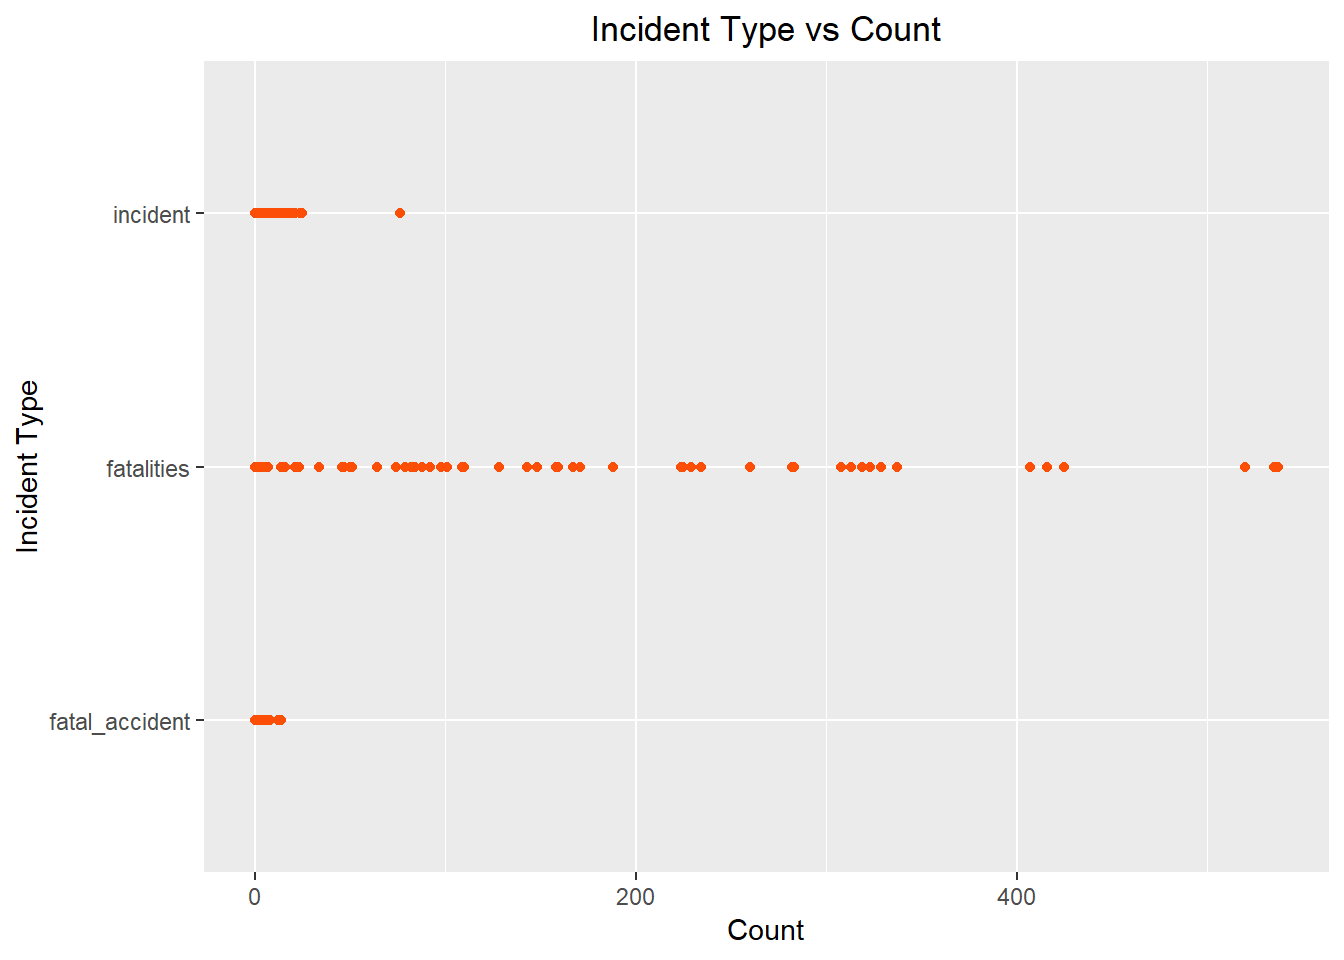
\includegraphics{data622hw1_files/figure-latex/unnamed-chunk-5-1.pdf}

\begin{Shaded}
\begin{Highlighting}[]
\NormalTok{m_glm <-}\StringTok{ }\KeywordTok{cbind}\NormalTok{(}\DataTypeTok{AUC=}\NormalTok{res}\OperatorTok{$}\NormalTok{stdres}\OperatorTok{$}\NormalTok{glm[}\StringTok{'AUC-ROC'}\NormalTok{,}\StringTok{'Score'}\NormalTok{], }\DataTypeTok{Accuracy =} \KeywordTok{mean}\NormalTok{(fit_glm}\OperatorTok{$}\NormalTok{results[,}\StringTok{'Accuracy'}\NormalTok{]), }\DataTypeTok{FPR=}\NormalTok{res}\OperatorTok{$}\NormalTok{stdres}\OperatorTok{$}\NormalTok{glm[}\StringTok{'FPR'}\NormalTok{,}\StringTok{'Score'}\NormalTok{], }\DataTypeTok{TPR =}\NormalTok{ res}\OperatorTok{$}\NormalTok{stdres}\OperatorTok{$}\NormalTok{glm[}\StringTok{'TP'}\NormalTok{,}\StringTok{'Score'}\NormalTok{]}\OperatorTok{/}\NormalTok{(res}\OperatorTok{$}\NormalTok{stdres}\OperatorTok{$}\NormalTok{glm[}\StringTok{'TP'}\NormalTok{,}\StringTok{'Score'}\NormalTok{]}\OperatorTok{+}\NormalTok{res}\OperatorTok{$}\NormalTok{stdres}\OperatorTok{$}\NormalTok{glm[}\StringTok{'FN'}\NormalTok{,}\StringTok{'Score'}\NormalTok{]), }\DataTypeTok{TNR=}\NormalTok{res}\OperatorTok{$}\NormalTok{stdres}\OperatorTok{$}\NormalTok{glm[}\StringTok{'TN'}\NormalTok{,}\StringTok{'Score'}\NormalTok{]}\OperatorTok{/}\NormalTok{(res}\OperatorTok{$}\NormalTok{stdres}\OperatorTok{$}\NormalTok{glm[}\StringTok{'TN'}\NormalTok{,}\StringTok{'Score'}\NormalTok{]}\OperatorTok{+}\NormalTok{res}\OperatorTok{$}\NormalTok{stdres}\OperatorTok{$}\NormalTok{glm[}\StringTok{'FP'}\NormalTok{,}\StringTok{'Score'}\NormalTok{]), }\DataTypeTok{FNR=}\NormalTok{res}\OperatorTok{$}\NormalTok{stdres}\OperatorTok{$}\NormalTok{glm[}\StringTok{'FN'}\NormalTok{,}\StringTok{'Score'}\NormalTok{]}\OperatorTok{/}\NormalTok{(res}\OperatorTok{$}\NormalTok{stdres}\OperatorTok{$}\NormalTok{glm[}\StringTok{'TP'}\NormalTok{,}\StringTok{'Score'}\NormalTok{]}\OperatorTok{+}\NormalTok{res}\OperatorTok{$}\NormalTok{stdres}\OperatorTok{$}\NormalTok{glm[}\StringTok{'FN'}\NormalTok{,}\StringTok{'Score'}\NormalTok{]))}

\NormalTok{m_nb <-}\StringTok{ }\KeywordTok{cbind}\NormalTok{(}\DataTypeTok{AUC=}\NormalTok{res}\OperatorTok{$}\NormalTok{stdres}\OperatorTok{$}\NormalTok{nb[}\StringTok{'AUC-ROC'}\NormalTok{,}\StringTok{'Score'}\NormalTok{],}\DataTypeTok{Accuracy =} \KeywordTok{mean}\NormalTok{(fit_nb}\OperatorTok{$}\NormalTok{results[,}\StringTok{'Accuracy'}\NormalTok{]), }\DataTypeTok{FPR=}\NormalTok{res}\OperatorTok{$}\NormalTok{stdres}\OperatorTok{$}\NormalTok{nb[}\StringTok{'FPR'}\NormalTok{,}\StringTok{'Score'}\NormalTok{],}\DataTypeTok{TPR =}\NormalTok{ res}\OperatorTok{$}\NormalTok{stdres}\OperatorTok{$}\NormalTok{nb[}\StringTok{'TP'}\NormalTok{,}\StringTok{'Score'}\NormalTok{]}\OperatorTok{/}\NormalTok{(res}\OperatorTok{$}\NormalTok{stdres}\OperatorTok{$}\NormalTok{nb[}\StringTok{'TP'}\NormalTok{,}\StringTok{'Score'}\NormalTok{]}\OperatorTok{+}\NormalTok{res}\OperatorTok{$}\NormalTok{stdres}\OperatorTok{$}\NormalTok{nb[}\StringTok{'FN'}\NormalTok{,}\StringTok{'Score'}\NormalTok{]), }\DataTypeTok{TNR=}\NormalTok{res}\OperatorTok{$}\NormalTok{stdres}\OperatorTok{$}\NormalTok{nb[}\StringTok{'TN'}\NormalTok{,}\StringTok{'Score'}\NormalTok{]}\OperatorTok{/}\NormalTok{(res}\OperatorTok{$}\NormalTok{stdres}\OperatorTok{$}\NormalTok{nb[}\StringTok{'TN'}\NormalTok{,}\StringTok{'Score'}\NormalTok{]}\OperatorTok{+}\NormalTok{res}\OperatorTok{$}\NormalTok{stdres}\OperatorTok{$}\NormalTok{nb[}\StringTok{'FP'}\NormalTok{,}\StringTok{'Score'}\NormalTok{]), }\DataTypeTok{FNR=}\NormalTok{res}\OperatorTok{$}\NormalTok{stdres}\OperatorTok{$}\NormalTok{nb[}\StringTok{'FN'}\NormalTok{,}\StringTok{'Score'}\NormalTok{]}\OperatorTok{/}\NormalTok{(res}\OperatorTok{$}\NormalTok{stdres}\OperatorTok{$}\NormalTok{nb[}\StringTok{'TP'}\NormalTok{,}\StringTok{'Score'}\NormalTok{]}\OperatorTok{+}\NormalTok{res}\OperatorTok{$}\NormalTok{stdres}\OperatorTok{$}\NormalTok{nb[}\StringTok{'FN'}\NormalTok{,}\StringTok{'Score'}\NormalTok{]))}

\NormalTok{m_knn <-}\StringTok{ }\KeywordTok{cbind}\NormalTok{(}\DataTypeTok{AUC=}\NormalTok{res}\OperatorTok{$}\NormalTok{stdres}\OperatorTok{$}\NormalTok{knn[}\StringTok{'AUC-ROC'}\NormalTok{,}\StringTok{'Score'}\NormalTok{], }\DataTypeTok{Accuracy =} \KeywordTok{mean}\NormalTok{(fit_knn}\OperatorTok{$}\NormalTok{results[,}\StringTok{'Accuracy'}\NormalTok{]), }\DataTypeTok{FPR=}\NormalTok{res}\OperatorTok{$}\NormalTok{stdres}\OperatorTok{$}\NormalTok{knn[}\StringTok{'FPR'}\NormalTok{,}\StringTok{'Score'}\NormalTok{],}\DataTypeTok{TPR =}\NormalTok{ res}\OperatorTok{$}\NormalTok{stdres}\OperatorTok{$}\NormalTok{knn[}\StringTok{'TP'}\NormalTok{,}\StringTok{'Score'}\NormalTok{]}\OperatorTok{/}\NormalTok{(res}\OperatorTok{$}\NormalTok{stdres}\OperatorTok{$}\NormalTok{knn[}\StringTok{'TP'}\NormalTok{,}\StringTok{'Score'}\NormalTok{]}\OperatorTok{+}\NormalTok{res}\OperatorTok{$}\NormalTok{stdres}\OperatorTok{$}\NormalTok{knn[}\StringTok{'FN'}\NormalTok{,}\StringTok{'Score'}\NormalTok{]), }\DataTypeTok{TNR=}\NormalTok{res}\OperatorTok{$}\NormalTok{stdres}\OperatorTok{$}\NormalTok{knn[}\StringTok{'TN'}\NormalTok{,}\StringTok{'Score'}\NormalTok{]}\OperatorTok{/}\NormalTok{(res}\OperatorTok{$}\NormalTok{stdres}\OperatorTok{$}\NormalTok{knn[}\StringTok{'TN'}\NormalTok{,}\StringTok{'Score'}\NormalTok{]}\OperatorTok{+}\NormalTok{res}\OperatorTok{$}\NormalTok{stdres}\OperatorTok{$}\NormalTok{knn[}\StringTok{'FP'}\NormalTok{,}\StringTok{'Score'}\NormalTok{]), }\DataTypeTok{FNR=}\NormalTok{res}\OperatorTok{$}\NormalTok{stdres}\OperatorTok{$}\NormalTok{knn[}\StringTok{'FN'}\NormalTok{,}\StringTok{'Score'}\NormalTok{]}\OperatorTok{/}\NormalTok{(res}\OperatorTok{$}\NormalTok{stdres}\OperatorTok{$}\NormalTok{knn[}\StringTok{'TP'}\NormalTok{,}\StringTok{'Score'}\NormalTok{]}\OperatorTok{+}\NormalTok{res}\OperatorTok{$}\NormalTok{stdres}\OperatorTok{$}\NormalTok{knn[}\StringTok{'FN'}\NormalTok{,}\StringTok{'Score'}\NormalTok{]))}
\end{Highlighting}
\end{Shaded}

\hypertarget{glm}{%
\subsubsection{GLM}\label{glm}}

\begin{Shaded}
\begin{Highlighting}[]
\NormalTok{m_glm}
\end{Highlighting}
\end{Shaded}

\begin{verbatim}
##       AUC  Accuracy   FPR       TPR       TNR       FNR
## [1,] 0.83 0.7340685 0.227 0.8571429 0.7727273 0.1428571
\end{verbatim}

\begin{Shaded}
\begin{Highlighting}[]
\KeywordTok{confusionMatrix}\NormalTok{(fit_glm)}
\end{Highlighting}
\end{Shaded}

\begin{verbatim}
## Bootstrapped (100 reps) Confusion Matrix 
## 
## (entries are percentual average cell counts across resamples)
##  
##           Reference
## Prediction BLACK BLUE
##      BLACK  46.9 10.3
##      BLUE   16.6 26.2
##                            
##  Accuracy (average) : 0.731
\end{verbatim}

\hypertarget{nb}{%
\subsubsection{NB}\label{nb}}

\begin{Shaded}
\begin{Highlighting}[]
\NormalTok{m_nb}
\end{Highlighting}
\end{Shaded}

\begin{verbatim}
##       AUC  Accuracy   FPR TPR       TNR FNR
## [1,] 0.94 0.6326558 0.591   1 0.4090909   0
\end{verbatim}

\begin{Shaded}
\begin{Highlighting}[]
\KeywordTok{confusionMatrix}\NormalTok{(fit_nb)}
\end{Highlighting}
\end{Shaded}

\begin{verbatim}
## Bootstrapped (100 reps) Confusion Matrix 
## 
## (entries are percentual average cell counts across resamples)
##  
##           Reference
## Prediction BLACK BLUE
##      BLACK  28.4  2.4
##      BLUE   32.8 36.5
##                             
##  Accuracy (average) : 0.6484
\end{verbatim}

\hypertarget{knn}{%
\subsubsection{KNN}\label{knn}}

\begin{Shaded}
\begin{Highlighting}[]
\NormalTok{m_knn}
\end{Highlighting}
\end{Shaded}

\begin{verbatim}
##       AUC  Accuracy   FPR       TPR       TNR       FNR
## [1,] 0.82 0.6830212 0.136 0.6428571 0.8636364 0.3571429
\end{verbatim}

\begin{Shaded}
\begin{Highlighting}[]
\KeywordTok{confusionMatrix}\NormalTok{(fit_knn)}
\end{Highlighting}
\end{Shaded}

\begin{verbatim}
## Bootstrapped (100 reps) Confusion Matrix 
## 
## (entries are percentual average cell counts across resamples)
##  
##           Reference
## Prediction BLACK BLUE
##      BLACK  49.0 18.4
##      BLUE   12.7 19.9
##                             
##  Accuracy (average) : 0.6894
\end{verbatim}

\begin{Shaded}
\begin{Highlighting}[]
\NormalTok{summary =}\StringTok{ }\KeywordTok{rbind}\NormalTok{(m_glm, m_nb, m_knn)}
\KeywordTok{rownames}\NormalTok{(summary) <-}\StringTok{ }\KeywordTok{c}\NormalTok{(}\StringTok{"LR"}\NormalTok{, }\StringTok{'NB'}\NormalTok{,}\StringTok{"KNN"}\NormalTok{)}
\NormalTok{summary}
\end{Highlighting}
\end{Shaded}

\begin{verbatim}
##      AUC  Accuracy   FPR       TPR       TNR       FNR
## LR  0.83 0.7340685 0.227 0.8571429 0.7727273 0.1428571
## NB  0.94 0.6326558 0.591 1.0000000 0.4090909 0.0000000
## KNN 0.82 0.6830212 0.136 0.6428571 0.8636364 0.3571429
\end{verbatim}

\hypertarget{conclusion}{%
\subsubsection{Conclusion}\label{conclusion}}

From the above matrix we see that LR has a high True Positive Rate (TPR)
and True negative Rate (TNR) and a smaller False Positive Rate (FPR) and
False Negative Rate (FNR). NB and KNN on the other hand have interesting
results. In the case of NB it has high TPR and a zero FNR but 60\% FPR.
KNN has 91\% TNR and a lower TPR compared to LR. So I would think LR is
a better model.

\hypertarget{visuals}{%
\subsection{Visuals}\label{visuals}}

\begin{Shaded}
\begin{Highlighting}[]
\NormalTok{res}\OperatorTok{$}\NormalTok{roc}
\end{Highlighting}
\end{Shaded}

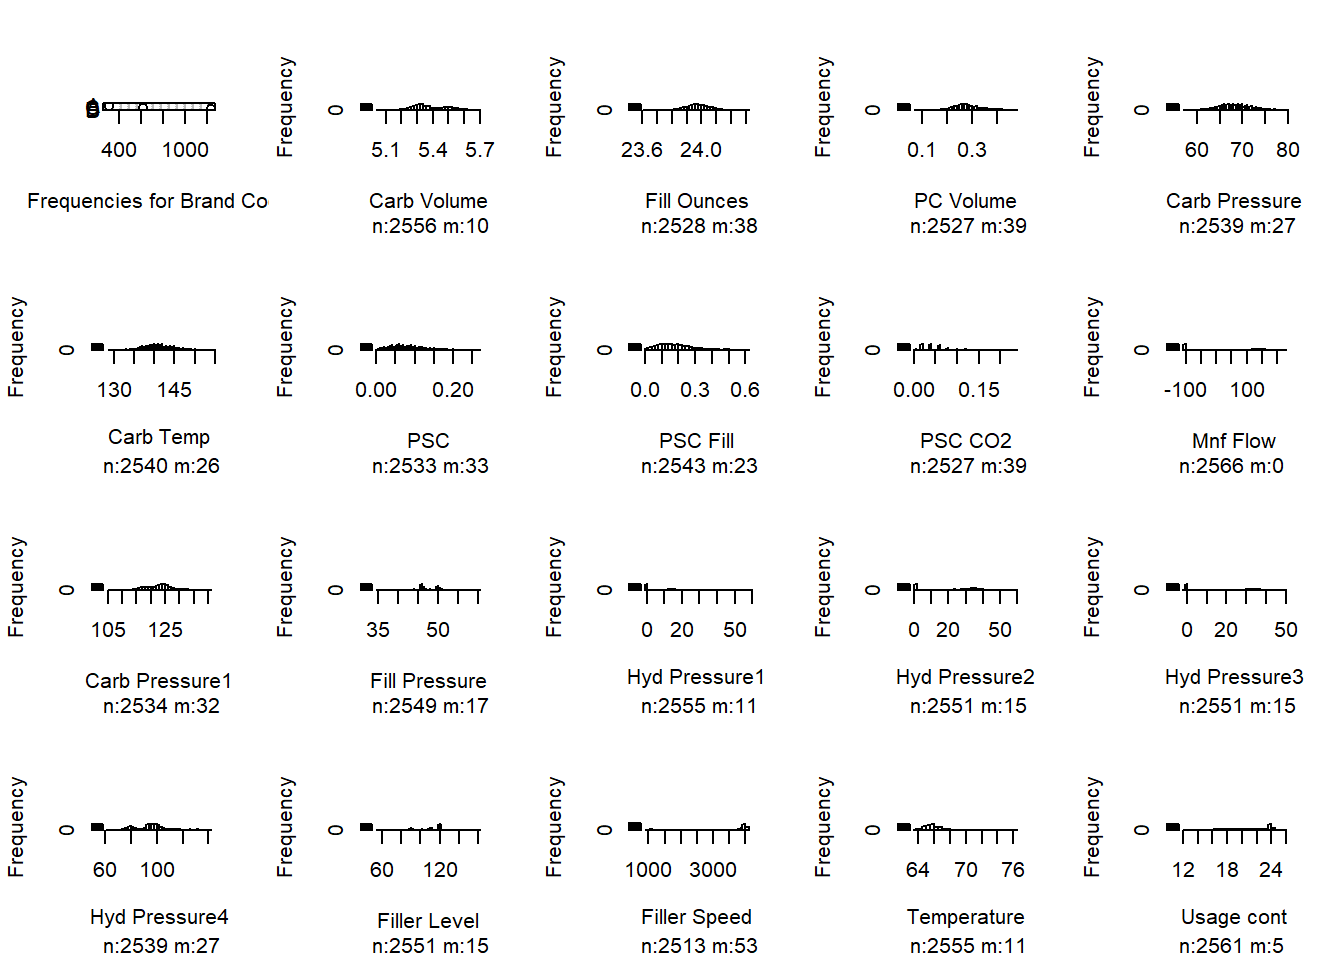
\includegraphics{data622hw1_files/figure-latex/unnamed-chunk-11-1.pdf}

\begin{Shaded}
\begin{Highlighting}[]
\NormalTok{res}\OperatorTok{$}\NormalTok{proc}
\end{Highlighting}
\end{Shaded}

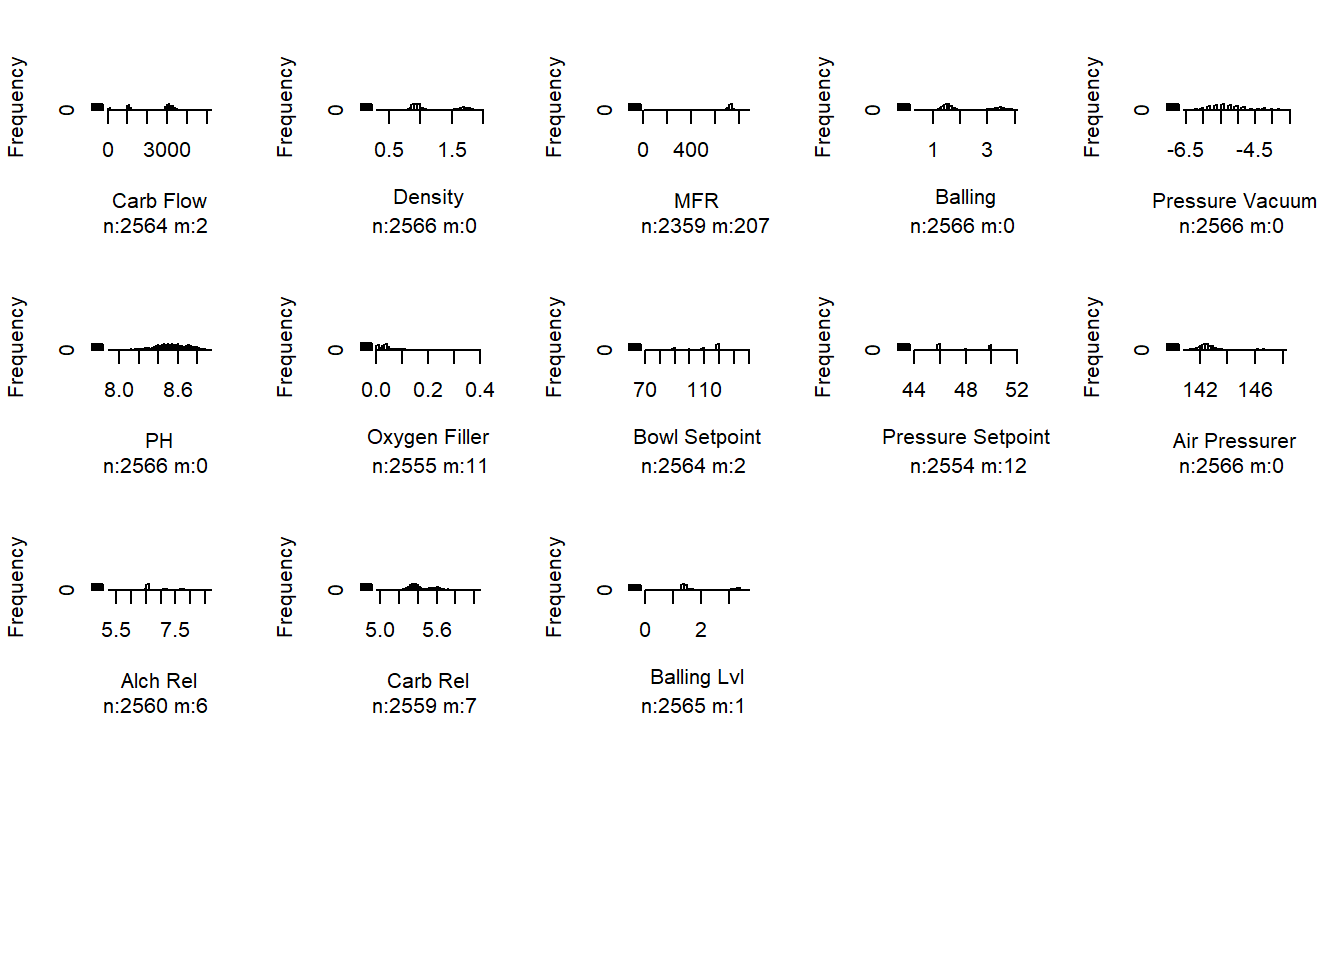
\includegraphics{data622hw1_files/figure-latex/unnamed-chunk-11-2.pdf}

\begin{Shaded}
\begin{Highlighting}[]
\NormalTok{res}\OperatorTok{$}\NormalTok{prg}
\end{Highlighting}
\end{Shaded}

\includegraphics{data622hw1_files/figure-latex/unnamed-chunk-11-3.pdf}

\begin{Shaded}
\begin{Highlighting}[]
\NormalTok{res}\OperatorTok{$}\NormalTok{cc}
\end{Highlighting}
\end{Shaded}

\includegraphics{data622hw1_files/figure-latex/unnamed-chunk-11-4.pdf}

\hypertarget{question-2}{%
\section{Question 2}\label{question-2}}

\hypertarget{what-aspects-of-the-data-and-or-aspects-of-the-algorithms-explain-these-performance-differences}{%
\paragraph{What aspects of the data and or aspects of the algorithms,
explain these performance
differences}\label{what-aspects-of-the-data-and-or-aspects-of-the-algorithms-explain-these-performance-differences}}

Linear Regression is a regression model, meaning, it'll take features
and predict a continuous output, eg : stock price,salary etc. Linear
regression as the name says, finds a linear curve solution to every
problem.

LR is easy and simple to implement. It is fast in training and is good
at space complex solution. LR however is applicable only if the solution
is linear. In many real life scenarios, it may not be the case. The
algorithm assumes the input residuals (error) to be normal distributed,
but may not be satisfied always. It assumes input features to be
mutually independent(no co-linearity).

Naive bayes is a generative model whereas LR is a discriminative model.
Naive bayes works well with small datasets, whereas LR+regularization
can achieve similar performance. LR performs better than naive bayes
upon colinearity, as naive bayes expects all features to be independent.

KNN is a non-parametric model, where LR is a parametric model. It is
comparatively slower than Logistic Regression. KNN supports non-linear
solutions where LR supports only linear solutions. LR can derive
confidence level (about its prediction), whereas KNN can only output the
labels. KNN is slow in real time as it have to keep track of all
training data and find the neighbor nodes, whereas LR can easily extract
output from the tuned θ coefficients.

\end{document}
